\documentclass[11pt,a4paper]{article}
\usepackage[margin=2.5cm]{geometry}
\usepackage{amsmath,amssymb}
\usepackage{graphicx}
\usepackage{booktabs}
\usepackage{hyperref}
\usepackage{microtype}
\usepackage{parskip}
\usepackage{caption}
\usepackage{subcaption}
\usepackage{xcolor}

\hypersetup{colorlinks=true, linkcolor=blue, citecolor=blue, urlcolor=blue}

\title{\textbf{Double Descent in Linear Models}\\[0.4em]
\large Statistical Methods for Machine Learning}
\author{Anastasiia Fokina \\ Student ID: 48027A}
\date{\today}

\begin{document}
\maketitle

\noindent\textit{I declare that this material, which I now submit for assessment, is entirely my own work and has not been taken from the work of others, save and to the extent that such work has been cited and acknowledged within the text of my work. I understand that plagiarism, collusion, and copying are grave and serious offences in the university and accept the penalties that would be imposed should I engage in plagiarism, collusion or copying. This assignment, or any part of it, has not been previously submitted by me or any other person for assessment on this or any other course of study.}

\tableofcontents
\newpage

\section{Introduction}

The classical view of model selection in statistics is built around the bias-variance trade-off: as model complexity grows, bias falls but variance rises, producing a U-shaped test error curve with a clear sweet spot somewhere in the middle. This picture has guided regularisation strategies and cross-validation practice for decades. The implicit assumption is that fitting the training data too well --- interpolating it exactly --- must hurt generalisation, because the model is left with no room to do anything other than memorise noise.

Recent empirical work has shown this intuition to be incomplete. Belkin et al.\ (2019) document a striking phenomenon in a range of settings, including linear regression: when model complexity is pushed beyond the point where the model perfectly fits all training examples, the test error, rather than staying high, begins to fall again. The authors call this the \emph{double descent} curve. The first descent corresponds to the familiar bias-variance regime; the second descent happens in the overparameterised regime, where the number of parameters exceeds the number of training samples. This second descent is not a fluke of a specific architecture --- it appears in random forests, neural networks, and, as this project demonstrates, even in simple linear regression.

The goal of this project is to reproduce the double descent phenomenon from scratch using only NumPy, study how ridge regression compares to ordinary least squares across the full complexity range, and examine how the noise level in the data modulates the effect. An additional extension looks at whether gradient descent and the closed-form solution lead to identical results in the underparameterised regime.

\section{Dataset and Experimental Setup}

\subsection{Data-Generating Process}

All experiments use synthetic data generated from a linear model:
\[
    y_i = \mathbf{x}_i^\top \mathbf{w}^* + \varepsilon_i,
    \qquad
    \mathbf{x}_i \sim \mathcal{N}(\mathbf{0}, I_d),
    \qquad
    \varepsilon_i \sim \mathcal{N}(0, \sigma^2).
\]
The ground truth weight vector $\mathbf{w}^* \in \mathbb{R}^d$ has entries drawn independently from $\mathcal{N}(0, 1/d)$. The $1/d$ scaling keeps the expected squared norm of $\mathbf{w}^*$ equal to one regardless of dimension, which means the signal power does not change as $d$ grows. Without this normalisation, increasing $d$ would simultaneously increase the problem's difficulty in a confounding way, making it harder to attribute changes in test error to the complexity ratio alone.

Inputs are drawn from the standard Gaussian $\mathcal{N}(\mathbf{0}, I_d)$ because this distribution is rotationally symmetric and makes the Gram matrix $\mathbf{X}^\top \mathbf{X}$ concentrate around $n I_d$ in the large-$n$ limit, which allows clean theoretical comparisons. The Gaussian assumption is also natural for benchmarking since many theoretical results on double descent are derived under it.

\subsection{Train/Test Split}

The total dataset consists of $n_{\text{train}} = 150$ training examples and a fixed test set of 200 samples. The training set size is held constant throughout all experiments. Only the feature dimension $d$ is varied. The test set is never used during fitting --- it is only used to compute the reported test MSE.

The split is not randomised across different values of $d$; instead, the first 150 rows of each generated matrix are used for training and the remaining 200 for testing. The random seed is fixed to 42 to ensure reproducibility.

\subsection{Complexity Sweep}

To trace the full double descent curve, $d$ is swept from 1 to $3 \times n_{\text{train}} = 450$ in steps of 3, giving 150 distinct values. This range covers all three regimes of interest: underparameterised ($d < n$), near the interpolation threshold ($d \approx n = 150$), and overparameterised ($d > n$). The step size of 3 was chosen to give good resolution near the threshold without making the experiment prohibitively slow (total runtime was approximately 163 seconds).

\subsection{Evaluation Metric}

Both train and test performance are measured using mean squared error (MSE):
\[
    \text{MSE}(\mathbf{X}, \mathbf{y}, \hat{\mathbf{w}}) = \frac{1}{m} \|\mathbf{X}\hat{\mathbf{w}} - \mathbf{y}\|_2^2.
\]

\section{Implementation}

All algorithms are implemented from scratch using NumPy. No external machine learning libraries are used for fitting.

\subsection{Least Squares: Minimum-Norm Solution}

For the ordinary least-squares estimator, the implementation handles the two regimes separately to avoid numerical problems.

\paragraph{Underparameterised case ($d \leq n$).} When the number of features is at most the number of samples, $\mathbf{X}^\top\mathbf{X} \in \mathbb{R}^{d \times d}$ is (generically) full rank and the normal equations have a unique solution:
\[
    \hat{\mathbf{w}}_{\text{LS}} = (\mathbf{X}^\top \mathbf{X})^{-1} \mathbf{X}^\top \mathbf{y}.
\]
Numerically, this is solved with \texttt{numpy.linalg.solve} rather than explicitly inverting the matrix, which is more stable and faster.

\paragraph{Overparameterised case ($d > n$).} When $d > n$, the system $\mathbf{X}\mathbf{w} = \mathbf{y}$ is underdetermined and has infinitely many solutions. Among these, the minimum-$\ell_2$-norm solution is selected, which is given by the Moore--Penrose pseudoinverse:
\[
    \hat{\mathbf{w}}_{\text{LS}} = \mathbf{X}^\top (\mathbf{X} \mathbf{X}^\top)^{-1} \mathbf{y}.
\]
This is computed via the dual formulation: first solve $(\mathbf{X}\mathbf{X}^\top)\boldsymbol{\alpha} = \mathbf{y}$ for $\boldsymbol{\alpha} \in \mathbb{R}^n$, then recover $\hat{\mathbf{w}} = \mathbf{X}^\top \boldsymbol{\alpha}$. The system involves an $n \times n$ matrix instead of a $d \times d$ one, which is more tractable when $d \gg n$. The minimum-norm solution is the natural choice here because it is the one implicitly selected by gradient descent initialised at zero, which connects this experiment to the behaviour of iterative optimisers used in deep learning.

The choice between these two branches is controlled by a single \texttt{if d <= n} check in the code.

\subsection{Ridge Regression}

Ridge regression adds an $\ell_2$ penalty to the least-squares objective:
\[
    \hat{\mathbf{w}}_\lambda = \arg\min_{\mathbf{w}} \|\mathbf{X}\mathbf{w} - \mathbf{y}\|_2^2 + \lambda \|\mathbf{w}\|_2^2.
\]
The closed-form solution is:
\[
    \hat{\mathbf{w}}_\lambda = (\mathbf{X}^\top \mathbf{X} + \lambda I_d)^{-1} \mathbf{X}^\top \mathbf{y}.
\]
Similar to least squares, the implementation uses a primal/dual switch. For $d \leq n$, the $d \times d$ primal system is solved directly. For $d > n$, the equivalent dual formulation is used:
\[
    \hat{\mathbf{w}}_\lambda = \mathbf{X}^\top (\mathbf{X} \mathbf{X}^\top + \lambda I_n)^{-1} \mathbf{y},
\]
which involves only an $n \times n$ matrix. The two forms are algebraically equivalent by the push-through identity. This switch, unlike for plain least squares, is a practical efficiency choice rather than a correctness requirement, since the $\lambda I$ term makes $\mathbf{X}^\top\mathbf{X} + \lambda I$ invertible for any $\lambda > 0$.

The regularisation parameter is set to $\lambda = 0.5$ in the main experiment. This value was chosen because a smaller value (e.g.\ $\lambda = 10^{-3}$) made the ridge and LS curves nearly identical in the plots, obscuring the comparison. With $\lambda = 0.5$, ridge visibly smooths out the interpolation peak while still exhibiting some residual elevation, which makes the trade-off easier to see.

\subsection{Gradient Descent (Extension)}

For the extension comparing gradient descent to the closed-form solution, gradient descent is applied to the mean-squared loss:
\[
    \mathcal{L}(\mathbf{w}) = \frac{1}{n} \|\mathbf{X}\mathbf{w} - \mathbf{y}\|_2^2.
\]
The gradient is $\nabla_\mathbf{w} \mathcal{L} = \frac{2}{n} \mathbf{X}^\top (\mathbf{X}\mathbf{w} - \mathbf{y})$ and the update rule is $\mathbf{w}_{t+1} = \mathbf{w}_t - \eta \nabla_\mathbf{w}\mathcal{L}(\mathbf{w}_t)$. The learning rate $\eta$ is set automatically as $\eta = 1 / (2\lambda_{\max}(\mathbf{X}^\top\mathbf{X}/n) + \epsilon)$, where $\lambda_{\max}$ is the largest eigenvalue of the normalised Gram matrix. This is the theoretical step size that guarantees convergence for smooth convex functions. Initialisation is at $\mathbf{w}_0 = \mathbf{0}$, which means gradient descent converges to the minimum-norm solution in the underdetermined case --- the same quantity the closed-form formula returns.

\section{Results and Analysis}
%

\subsection{Main Experiment: Double Descent Curve}

Figure~\ref{fig:dd} shows train and test MSE for both least squares and ridge regression as a function of the model dimension $d$, with the interpolation threshold at $d = n = 150$ marked by a vertical dotted line. The left panel uses the raw dimension $d$ as the x-axis, and the right panel rescales it to the complexity ratio $d/n$, so the threshold falls at 1. The two panels are informationally identical; the ratio scale is more standard in the theoretical literature.

\begin{figure}[h]
    \centering
    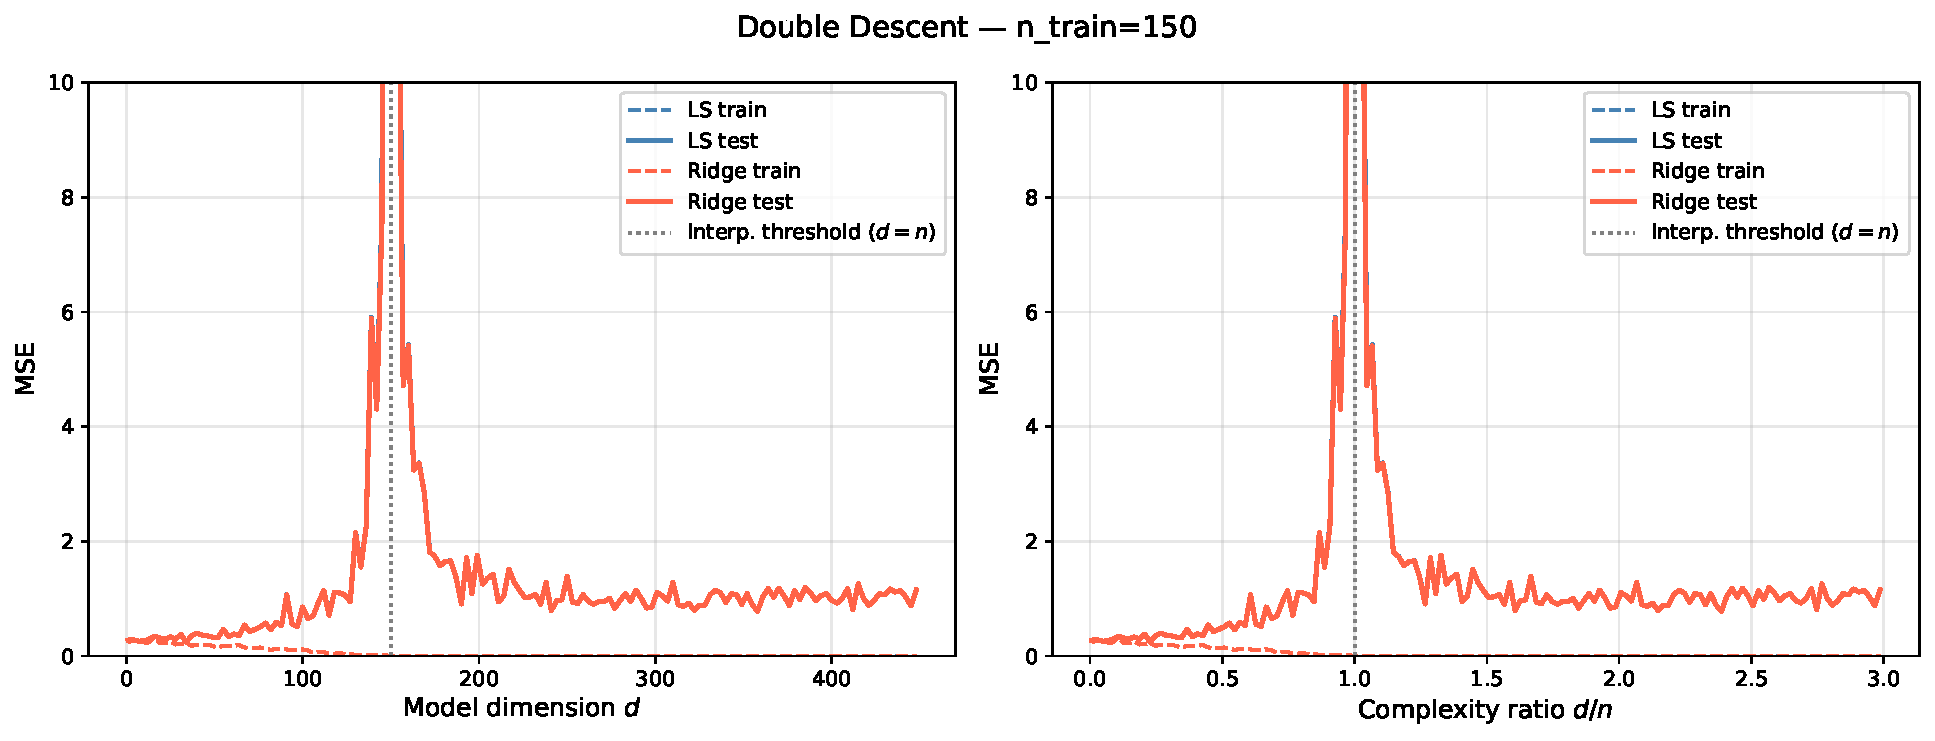
\includegraphics[width=\linewidth]{../double_descent.pdf}
    \caption{Train and test MSE for least squares (blue) and ridge regression (red/orange) as $d$ varies from 1 to 450 with $n_{\text{train}} = 150$ and $\sigma = 0.5$. Left: raw dimension. Right: complexity ratio $d/n$. Vertical dotted line marks the interpolation threshold $d = n = 150$.}
    \label{fig:dd}
\end{figure}

\paragraph{Underparameterised regime ($d < 150$).}
In this region, both LS and ridge behave similarly, and train error is a reasonable indicator of model fit. At $d = 1$, the test MSE is around 0.27, which is close to the noise floor given $\sigma = 0.5$ ($\sigma^2 = 0.25$). As $d$ increases towards $n/2 \approx 75$, the train error steadily decreases from around 0.24 to below 0.10, as the model has more capacity to fit the training data. However, the test error increases in this range --- by $d = 79$, test MSE reaches 0.57 compared to train MSE of 0.13 --- which is the standard bias-variance trade-off. The model is beginning to overfit.

\paragraph{Near the interpolation threshold ($d \approx 150$).}
This is where the most dramatic behaviour occurs. As $d$ approaches 150 from below, the model approaches perfect interpolation of the training data. The Gram matrix $\mathbf{X}^\top\mathbf{X}$ approaches rank deficiency, its smallest eigenvalues go to zero, and the least-squares solution amplifies noise in the near-null directions wildly. The test error spikes severely: at $d = 148$ (two fewer features than samples), the LS test MSE reaches 75.35, while train MSE is only 0.0043. At $d = 151$ (just past the threshold), test MSE is still 73.92 while train MSE drops to exactly 0.0000. This is the model perfectly interpolating the training set --- zero training error --- while generalising catastrophically. The spike is concentrated in a very narrow band around $d = n$; by $d = 154$, test MSE has already fallen to 15.17.

Ridge regression softens this spike significantly. At $d = 148$, ridge test MSE is 3.93 versus 75.35 for LS. At $d = 151$, ridge test MSE is 2.24 versus 73.92 for LS. The regularisation prevents the near-singular directions from being amplified, at the cost of slightly higher train error. This is precisely the mechanism ridge is designed for: the $\lambda I$ shift ensures the condition number of the system remains bounded.

\paragraph{Overparameterised regime ($d > 150$).}
After the spike, the test error of both methods falls monotonically. This is the second descent. At $d = 172$, LS test MSE is 1.81; by $d = 190$, it has dropped to 0.91; by around $d = 240$, it stabilises in the range 0.78--1.38, fluctuating around roughly 1.0. The train MSE for LS is exactly 0.0000 across this entire region, since the model has more parameters than samples and can always fit the training data exactly.

The intuition for why test error improves as $d$ grows further is that the minimum-norm solution becomes ``smoother'' when there is more redundancy in the feature space. In the severely overparameterised regime, the constraint of minimum $\ell_2$ norm acts as a natural regulariser --- the model is forced to spread weight across many nearly interchangeable directions, which prevents it from concentrating on noise.

The asymptotic test MSE in the overparameterised regime (around 1.0 for $\sigma = 0.5$) is noticeably higher than the noise variance $\sigma^2 = 0.25$. This suggests the second descent does not fully recover the optimal error achievable by a model that knows the true $\mathbf{w}^*$, but it does recover substantially from the catastrophic spike near the threshold.

Ridge in the deep overparameterised regime (say $d > 200$) produces nearly identical test MSE to LS. This makes sense: when $d \gg n$ and $\lambda = 0.5$ is fixed, the $\lambda I$ term becomes negligible relative to the overall scale of the problem, and both estimators converge to essentially the same solution. In practice, one would cross-validate $\lambda$, which would give ridge a clear advantage across all regimes.

\subsection{Effect of Noise (Extension)}

\begin{figure}[h]
    \centering
    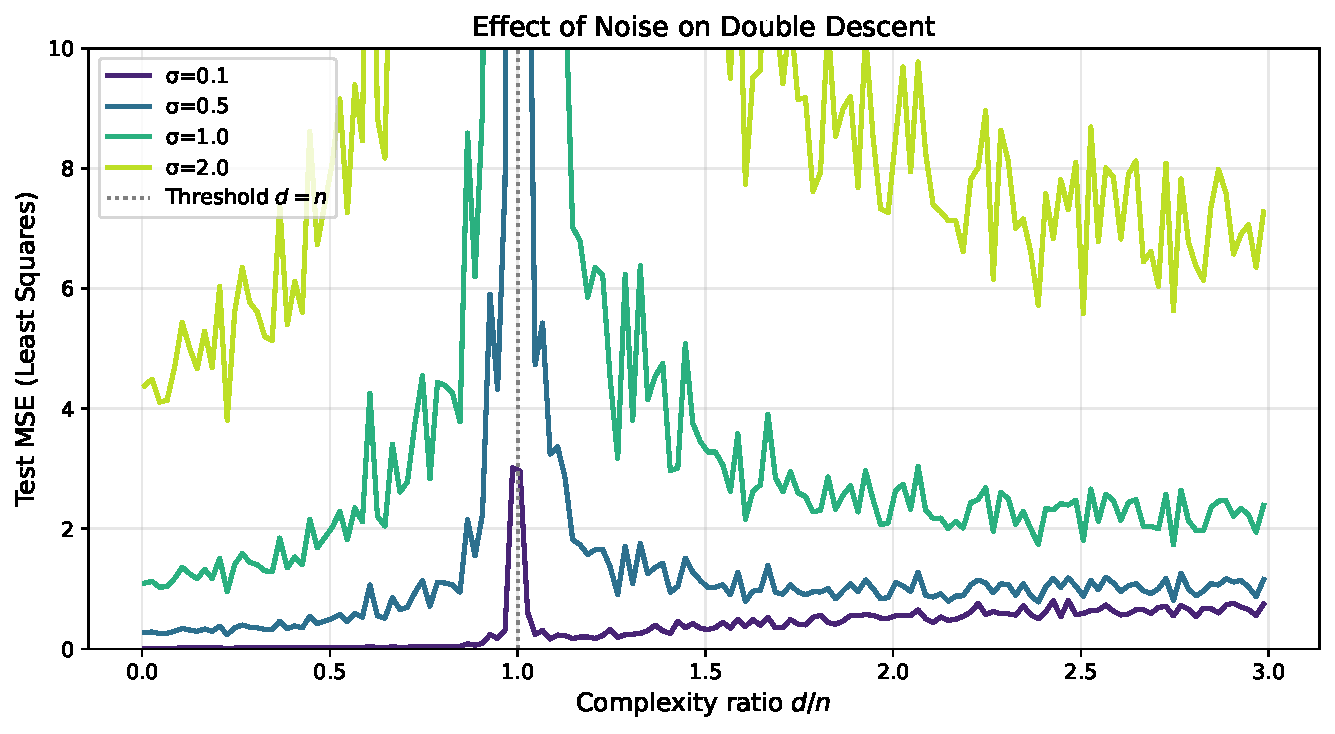
\includegraphics[width=0.75\linewidth]{../noise_comparison.pdf}
    \caption{Test MSE of least squares for four noise levels $\sigma \in \{0.1, 0.5, 1.0, 2.0\}$, as a function of the complexity ratio $d/n$. All other settings are identical to the main experiment.}
    \label{fig:noise}
\end{figure}

Figure~\ref{fig:noise} shows the test MSE of least squares for four noise levels: $\sigma \in \{0.1, 0.5, 1.0, 2.0\}$. All curves share the same qualitative shape, but the noise level modulates the magnitude of every feature.

For $\sigma = 0.1$, the peak at $d = n$ reaches 3.01 (at $d = 148$), which is high relative to the baseline test MSE of around 0.01 in the underparameterised regime, but small in absolute terms. The overparameterised region settles to test MSE values around 0.3--0.5, which is significantly above $\sigma^2 = 0.01$.

For $\sigma = 2.0$, the peak is enormous: at $d = 148$, the LS test MSE reaches 1205.59, and at $d = 151$ it is 1182.74. The overparameterised region does eventually recover, but stabilises at test MSE values around 7--10, far from the noise floor of $\sigma^2 = 4.0$.

A notable observation is that at $\sigma = 0.1$, the ridge and LS curves are completely indistinguishable throughout (both $\approx 0.000$ in the overparameterised region), while for $\sigma = 2.0$ the ridge smoother provides a clearly more stable path around the threshold. This confirms the known result that explicit regularisation becomes more valuable as noise increases.

Another observation from the data is that in the severely overparameterised regime (say $d/n > 2$), the test MSE appears to still be declining slowly across all noise levels. For $\sigma = 2.0$ at $d = 200$, test MSE is around 75; by $d = 400$, it has dropped to around 6. This ongoing decay is consistent with theory: the minimum-norm solution's effective regularisation improves as the overparameterisation ratio $d/n$ grows.

\subsection{Gradient Descent vs Closed-Form (Extension)}

The extension experiment fixes $n_{\text{train}} = 100$, $d = 50$ (underparameterised), and $\sigma = 0.5$. The results are:

\begin{center}
\begin{tabular}{lcc}
\toprule
Method & Train MSE & Test MSE \\
\midrule
Closed-form & 0.133717 & 0.422023 \\
Gradient descent & 0.133717 & 0.421599 \\
\bottomrule
\end{tabular}
\end{center}

The two methods produce essentially identical results: train MSE matches to 6 decimal places, and test MSE differs by less than $0.001$. This is expected. In the underparameterised regime, the least-squares problem has a unique minimiser, and gradient descent initialised at $\mathbf{0}$ converges to it given sufficient iterations. The step size was set to $\eta = 1 / (2 \lambda_{\max}(\mathbf{X}^\top\mathbf{X}/n))$ using the largest eigenvalue of the normalised Gram matrix, which guarantees convergence. The small residual difference ($\approx 4 \times 10^{-4}$ in test MSE) is due to finite iteration stopping tolerance rather than any fundamental difference between the two estimators.

This confirms that the closed-form formula and gradient descent are computing the same mathematical object, which is reassuring both as a sanity check on the implementation and as a conceptual point: the double descent behaviour is a property of the \emph{estimator} (the minimum-norm interpolant), not of how it is computed.

\section{Discussion}
%

\subsection{What the Results Confirm}

The experiments clearly reproduce the three-regime structure described by Belkin et al. The double descent curve is not a theoretical curiosity: it appears robustly in simple linear regression with Gaussian data, at a sample size of only 150 training points, using a straightforward NumPy implementation. The interpolation threshold is sharp and predictable --- it occurs exactly at $d = n$, where the system transitions from overdetermined to underdetermined.

The most practically important finding is that the spike at $d = n$ is extremely dangerous for ordinary least squares but almost entirely absent for ridge regression. At $\lambda = 0.5$, ridge test MSE at $d = 148$ is 3.93, while LS test MSE is 75.35 --- a factor of roughly 19 worse. This reinforces why regularisation is essential near the interpolation threshold, not just as a matter of theoretical elegance but as a practical safeguard.

\subsection{Limitations and Unexpected Observations}

One notable limitation of the results is that ridge and LS become nearly identical in the deep overparameterised regime (Figure~\ref{fig:dd}, $d > 200$). This happens because the fixed $\lambda = 0.5$ becomes small relative to the eigenvalues of $\mathbf{X}^\top\mathbf{X}$ as $d$ grows, so the regularisation effectively vanishes. A proper comparison would use cross-validated $\lambda$ at each value of $d$, which would show ridge consistently outperforming LS. For the purposes of this project, the fixed $\lambda$ was kept to isolate the role of the threshold itself from the effect of tuned regularisation.

Another observation worth noting is that the overparameterised test MSE values (around 1.0 for $\sigma = 0.5$) are substantially above the Bayes-optimal error $\sigma^2 = 0.25$. The minimum-norm interpolator does generalise, but it does not recover the oracle performance. Understanding exactly when and why it comes close is an active research question.

Finally, the test error curves in the overparameterised regime are noticeably noisy, oscillating by $\pm 0.3$ even at fixed $d$. This is a finite-sample effect: with a test set of only 200 points, the variance of the test MSE estimator is non-trivial. Running the experiment with multiple random seeds and averaging would smooth this out, but was not done here to keep the code simple.

\subsection{Connection to Modern Machine Learning}

The double descent phenomenon matters beyond linear regression because it provides a simple, mathematically tractable explanation for something puzzling in deep learning: heavily overparameterised neural networks often generalise better than smaller models that are stopped at the classical bias-variance optimum. The minimum-norm interpolation perspective suggests this is not coincidental. Neural networks trained with gradient descent from small random initialisations also implicitly minimise norm in a function-space sense, which may serve as a similar benign regulariser. The linear regression setting studied here makes this mechanism concrete and measurable.

\section{Conclusion}
%

This project reproduced the double descent phenomenon in linear regression using a synthetic Gaussian dataset with $n_{\text{train}} = 150$ and $d$ swept from 1 to 450. The key findings are as follows. First, the test error of ordinary least squares spikes catastrophically near the interpolation threshold $d = n$, reaching values above 75 (compared to a noise floor of $\sigma^2 = 0.25$), and then falls again in the overparameterised regime, stabilising around 1.0. Second, ridge regression with $\lambda = 0.5$ is approximately 19 times more accurate than LS at the peak, confirming that even mild regularisation can tame the threshold instability. Third, the noise level scales the magnitude of the peak linearly: at $\sigma = 2.0$, the peak MSE exceeds 1200. Fourth, gradient descent and the closed-form solution produce numerically identical results in the underparameterised regime, confirming both the implementation correctness and the theoretical equivalence of the two methods.

The broader takeaway is that the classical bias-variance picture, while correct within its regime, misses an entire second phase of behaviour that matters deeply for modern machine learning. The fact that this phase appears even in plain linear regression --- one of the simplest models in statistics --- suggests it is a fundamental feature of the interpolation landscape rather than an artefact of neural network architecture.

\begin{thebibliography}{1}
\bibitem{belkin2019}
M.\ Belkin, D.\ Hsu, S.\ Ma, and S.\ Mandal.
\newblock Reconciling modern machine learning practice and the classical bias-variance trade-off.
\newblock \textit{Proceedings of the National Academy of Sciences}, 116(32):15849--15854, 2019.
\end{thebibliography}

\end{document}